\begin{frame}{Orientation}{}
\centering
\begin{figure}[!htb]%
    \subfloat{
        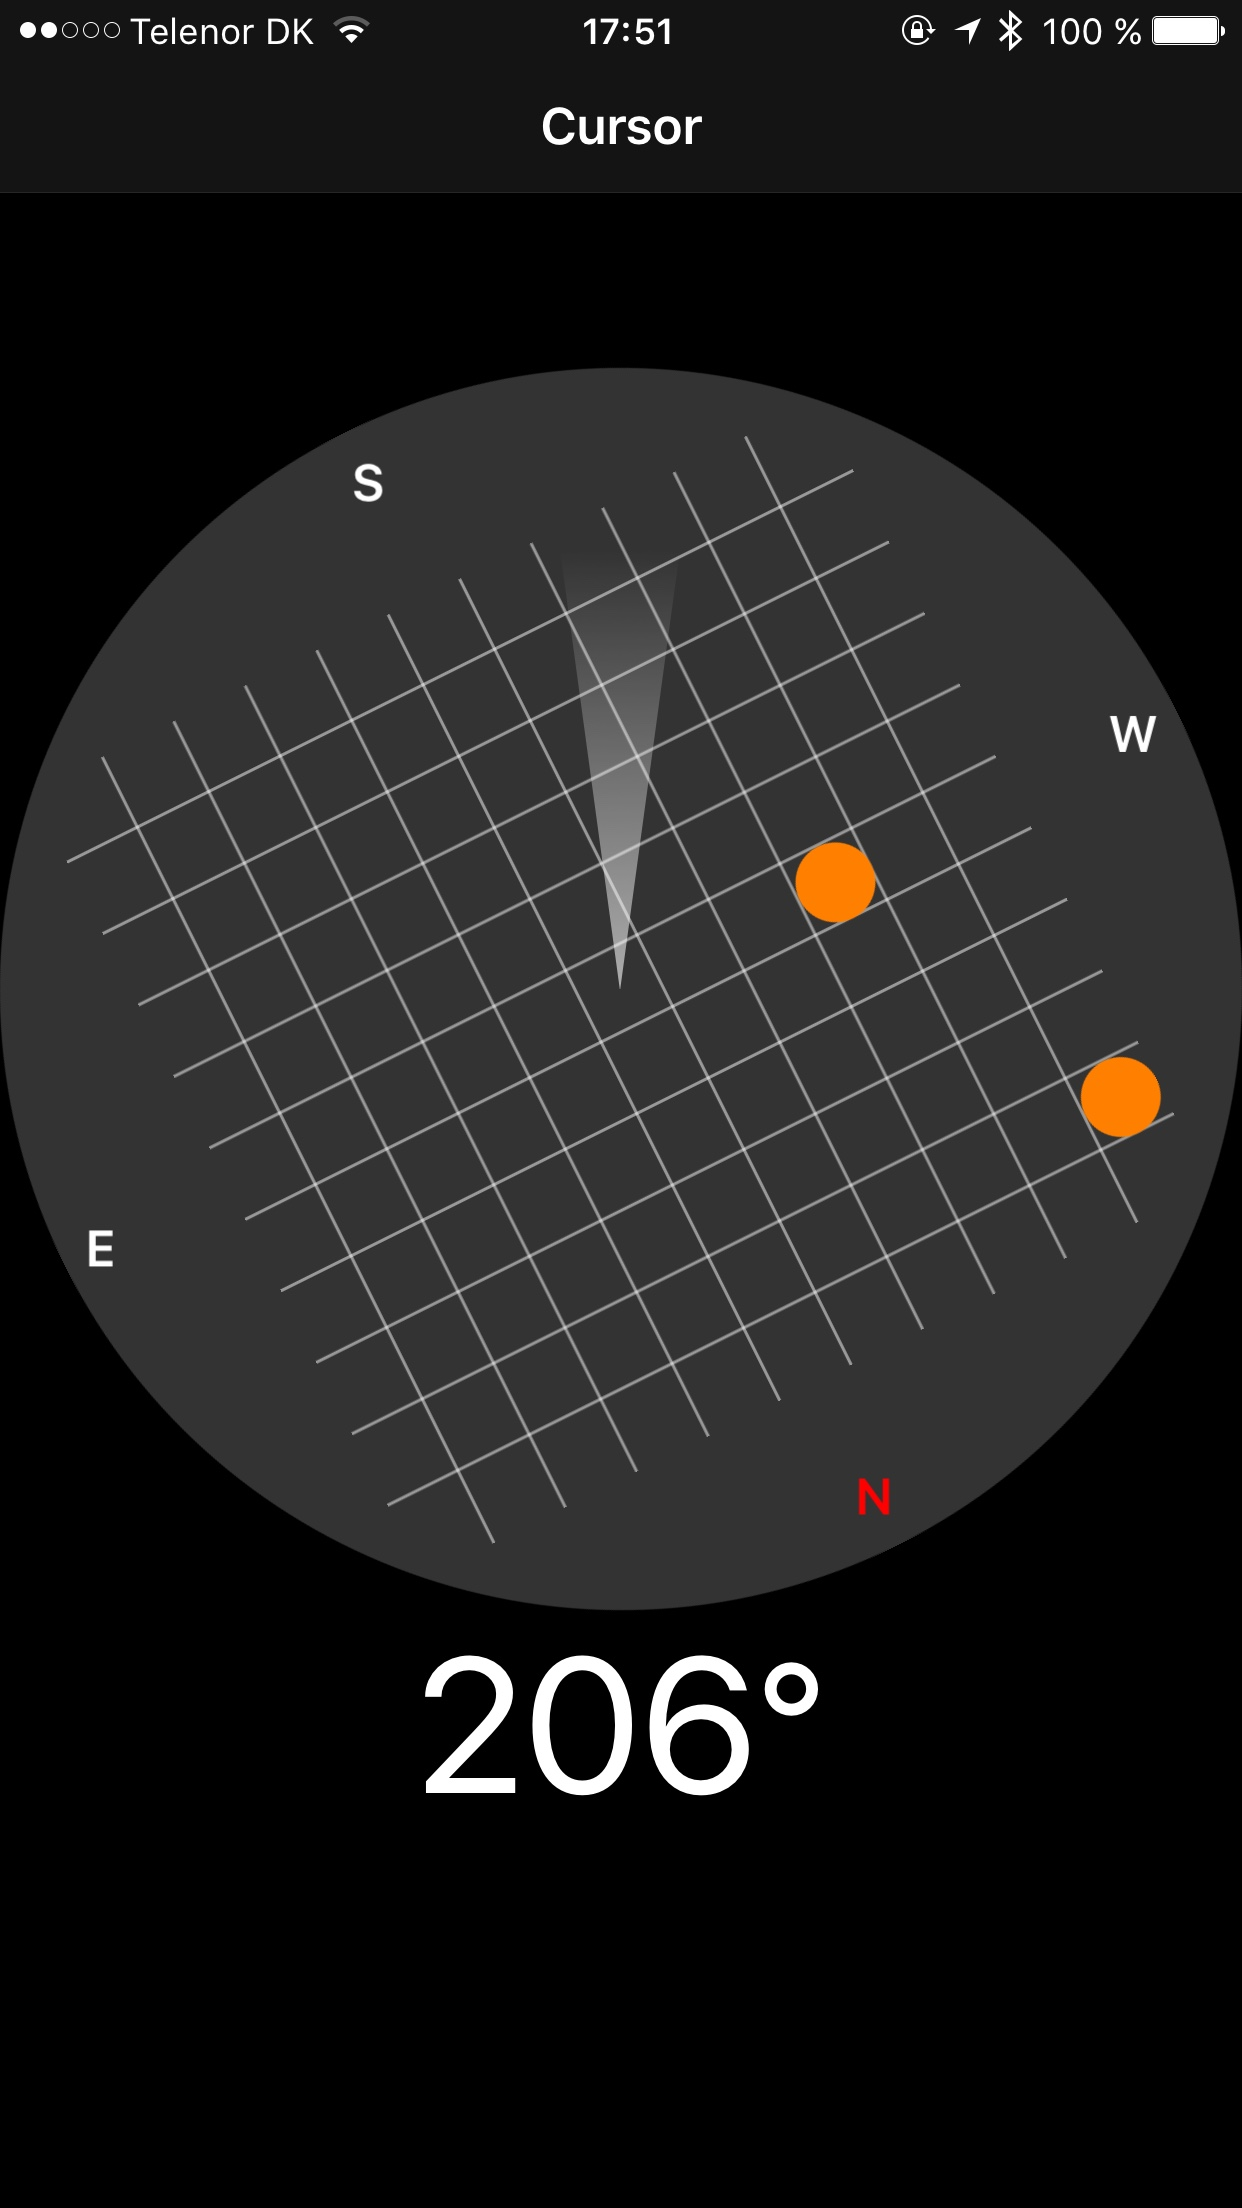
\includegraphics[width=0.25\textwidth]{../images/Prototype2_iOS_1.png}
    }
    \subfloat{
        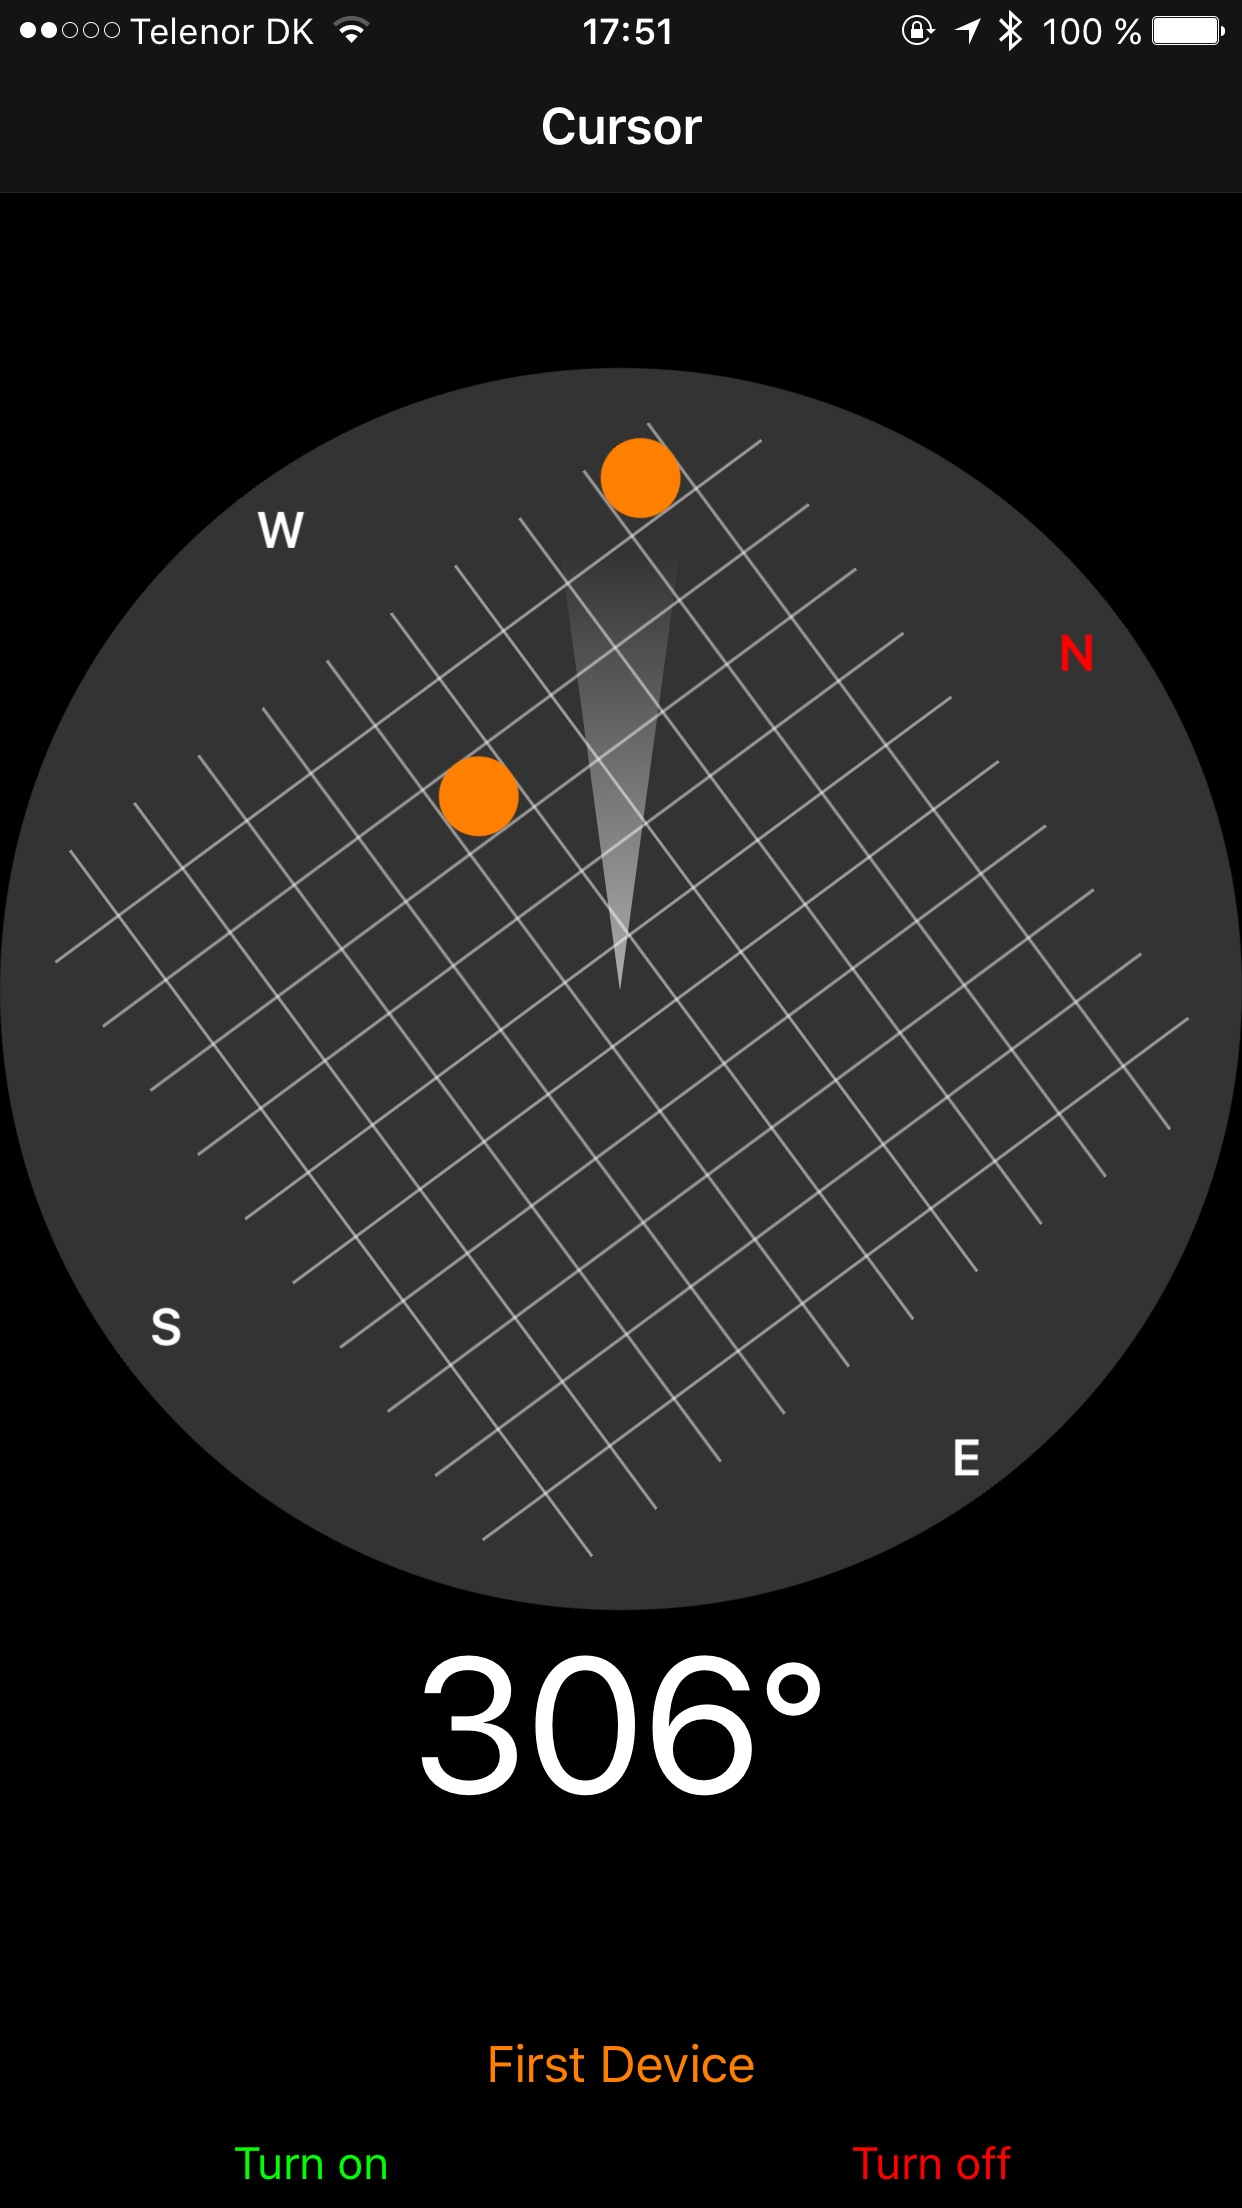
\includegraphics[width=0.25\textwidth]{../images/Prototype2_iOS_2.png}
    }
    \caption{Screenshots of the second prototype application. The white cone emitted from the center of the circle represents the area that the user is pointing at.}
\label{fig:prototype2-app-screenshots}
\end{figure}
\end{frame}

\begin{frame}{Orientation}{}
\centering
\begin{figure}[!htb]
    \centering
    \def\svgwidth{0.7\textwidth}
    \import{../drawings/}{../drawings/visibilityangle.pdf_tex}
    \caption{Finding objects in the visibility range. Device 1 is within the range, but Device 2 is not.}
\label{fig:visibilityangle}
\end{figure}
\end{frame}